\section{Схемотехнический анализ \\
  радиоэлектронного средства}

% Рассказывается про то как функционирует устройство, на основании того
% как объяснено функционирование принципиальной схемы, взятой из
% журнала. Приведен расчёт электрических параметров потенциометров и
% транзистора из схемы. Расчёт именно этих параметров обоснован тем, что
% они будут необходимы в дальнейшем для расчёта выделяемой теплоты.
% Возможно, будет использован САПР \textit{SimulIDE} вместо расчёта
% схемы в ручную.

\subsection{Описание принципа работы \\
  проектируемого радиоэлектронного средства.}

Поскольку статья о тестовом сервотестере написана в иностранном
журнале, схема электрическая принципиальная в нём выполнена не по
отечественному ГОСТ.

\begin{figure}[H]
  \centering
  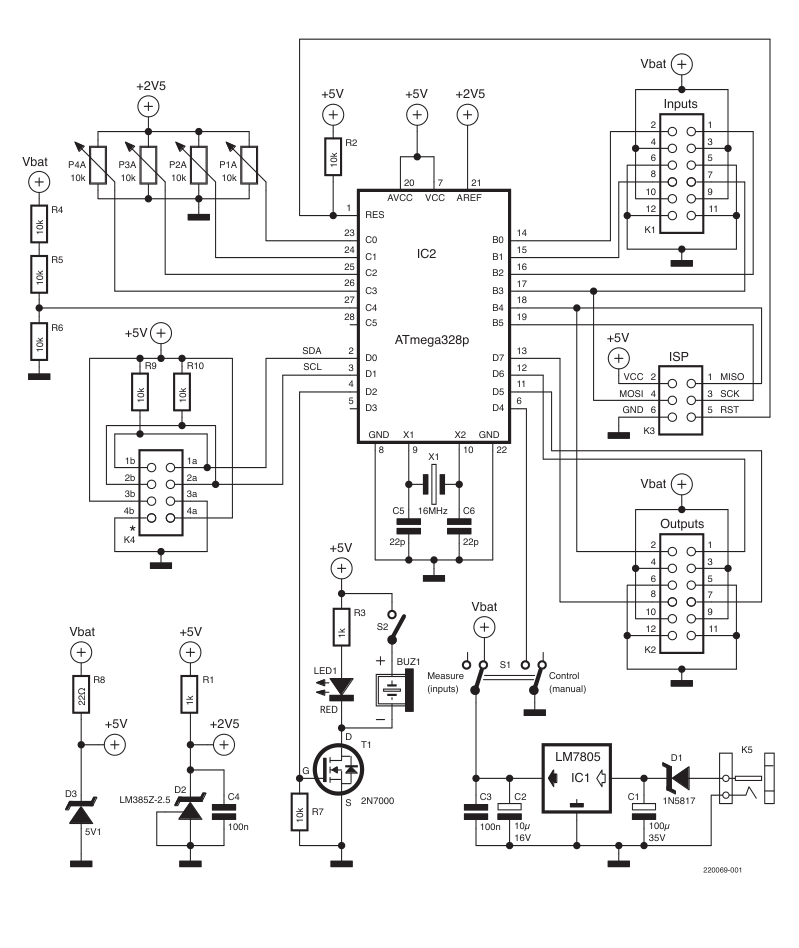
\includegraphics[scale = 0.50]{SchematicsShotFromElector.png}
  \caption{Электрическая принципиальная схема устройства}
\end{figure}

На приложенной схеме в центре видно микроконтроллер подключенный к
кристаллу с частотой колебаний 16 Мгц, который в свою очередь
подключен к конденсаторам C5 и С6. Четыре пина \textit{GPIO} — PB0-PB3
подключены к разъёму K1. Выводы для серво сигнала — PD5, PD6, PD7 и
PB4 подключены к разъёму K2. Два этих разъёма разведены таким
образом, что к ним можно подключить стандартный для сервопривода
кабель ~\cite{Elector521}.

Четыре потенциометра подключены к аналоговым входам микроконтроллера
PC0-PC3. Питание подключается через делитель напряжения из резисторов
R4-R6 к аналоговому входу PC4. Отношение между суммой сопротивлений
R4, R5 и сопротивлением R6 должно быть 2 к 1 соответственно, но их
абсолютные значения не критичны. Использование трёх резисторов одного
значения облегчает их сортировку для точности ~\cite{Elector521}.

Для того чтобы измерять напряжение источника питания нужен аналогово
цифровой преобразователь и опорное напряжение не относящиеся к самому
напряжению питания.  В микроконтроллере уже есть опорное напряжение в
1,1 Вольт, однако это значение несколько мало. И поэтому используется
источник опорного напряжения LM385-2.5 обозначенный как D2, как
внешнее опорное напряжение в 2,5 Вольта. Этот элемент более точен, чем
простой двух контактный зенеровский диод ~\cite{Elector521}.

К коннектору K4 подключается \textit{OLED} дисплей по типу SSD1306.  У
дисплея должен быть порт \textit{I2C}, но он будет подключаться к
порту \textit{I2C} микроконтроллера, но к компонентам PD0 и PD1. Шина
\textit{I2C} эмулируется программным обеспечением. Так выходит из-за
того, что шина \textit{I2C} на данном микроконтроллере находится на
том же пине, что и аналоговый вход PC4, который уже используется для
измерения напряжения питания ~\cite{Elector521}.

Резисторы R9 и R10 это подтягивающие резисторы для шины \textit{I2C}.

Ползунковый переключатель S1 типа \textit{DPDT} используется для
выбора режима работы сервотестера. В ручном режиме переключатель
соединяет напряжения питания номиналом 5 Вольт и коннекторы
сервоприводов. В режиме ввода он предотвращает неправильное включение
напряжений ~\cite{Elector521}.

Cама по себе схема достаточно проста,состоит из небольшого числа
компонентов, но тем не менее может работать в нескольких режимах и
схемах включения, что выглядит как положительные черты относительно
того в каких вариантах использования оказывается устройство.

\subsection{Расчет электрических параметров \\
  и режимов работы \\
  отдельных каскадов проектируемого устройства}

% Виктор Сильвестрович сказал здесь вставить расчет куска схемы с пищалкой

\newpage
%%% Local Variables:
%%% mode: LaTeX
%%% TeX-master: "main"
%%% End:
